\documentclass[10pt]{beamer}
\usetheme{AnnArbor}

\tolerance 99999
\hbadness 99999

\usepackage{amsmath,amsthm,amssymb,color,latexsym}
\usepackage{cancel}
\usepackage{graphicx}
\graphicspath{{images/}}
\setbeamertemplate{items}[ball]

\setbeamertemplate{footnote}{%
  \parindent 1em\noindent%
  \raggedright
  \insertfootnotetext\par%
}
\newcommand{\la}{\mathcal{L}}
\newcommand{\ma}{\mathcal{M}}
\newcommand{\ua}{\mathcal{U}}

\hypersetup{
  colorlinks,
  allcolors=.,
  urlcolor=blue,
}


\newenvironment{points}{\vspace{0.3cm} \begin{enumerate}[label={(\alph*)}]}{\end{enumerate} \vspace{0.2cm}}

\title{Masked Particle Modelling}
\subtitle{\textbf{CCNSB Seminar}}

\author[Abhiram Tilak]
{\textbf{Abhiram Tilak}}

\institute[IIITH]
{
	\textit{	\tiny{CND Dual Degree}} \\
	\textit{IIIT Hyderabad}
}


\date{October 14, 2024}

\begin{document}

\begin{frame}
	\titlepage
\end{frame}

\begin{frame}
\frametitle{Table of Contents}
\tableofcontents
\end{frame}

\begin{frame}{Introduction}
    This paper proposes a self-supervised model which uses unordered sets of
    particles with paramters as input and aims to build a generic
    foundational model.

    \begin{itemize}[<+->]
        \item The aim is to use this large foundation model and fine-tune it to
            be used in variety of down-stream tasks.
        \item Proposes a masking strategy based on models like BERT and BEiT
            to mask a set of particles in each jet.
        \item The model that is built should be capable of inferring the
            original particles using the information from other particles.
    \end{itemize}
\end{frame}

\section{Introduction}
\begin{frame}
    \begin{figure}
        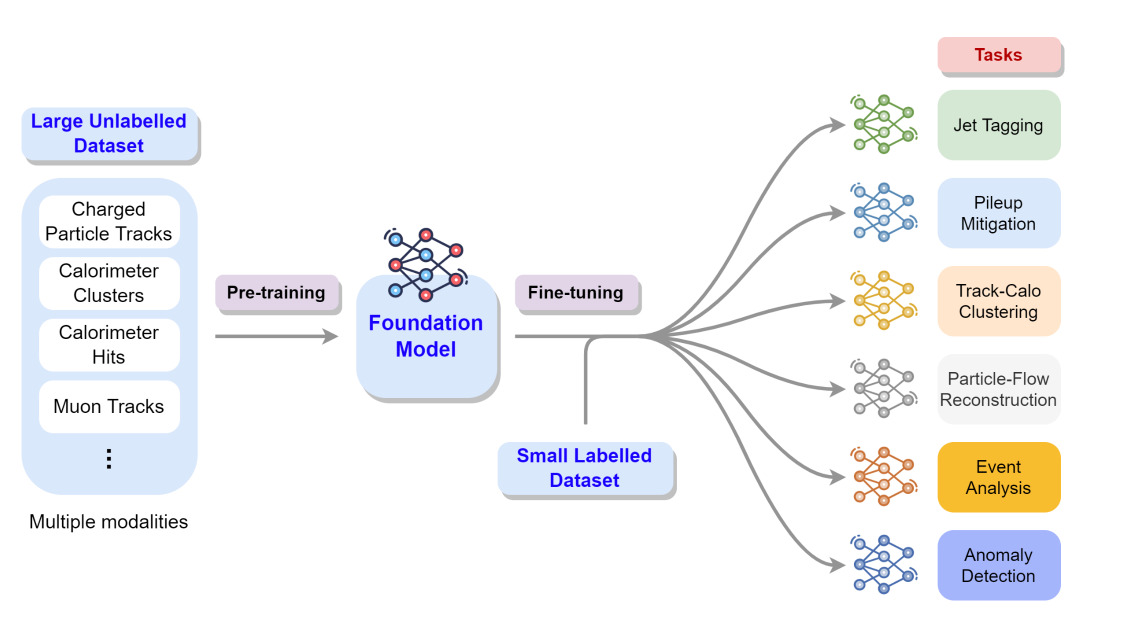
\includegraphics[width=0.9\textwidth]{intro.jpeg}
        \caption{Overview of the proposed Large foundation Model}
    \end{figure}
\end{frame}

\section{Background}
\begin{frame}{Background}
    The idea of masking in MPM comes from Masked Language Models widely used in
    the NLP and Computer Vision. Some of those popular models commnoly referred are:
    \begin{itemize}
        \item BERT (Bidirectional Encoder Representation from Transformers):

            \small
            BERT is a language
            model introduced in October 2018 by researchers at Google. It learns to
            represent text as a sequence of vectors using self-supervised learning. It uses
            the encoder-only transformer architecture.
            \begin{columns}
                \begin{column}{0.5\textwidth}
                    \begin{figure}
                        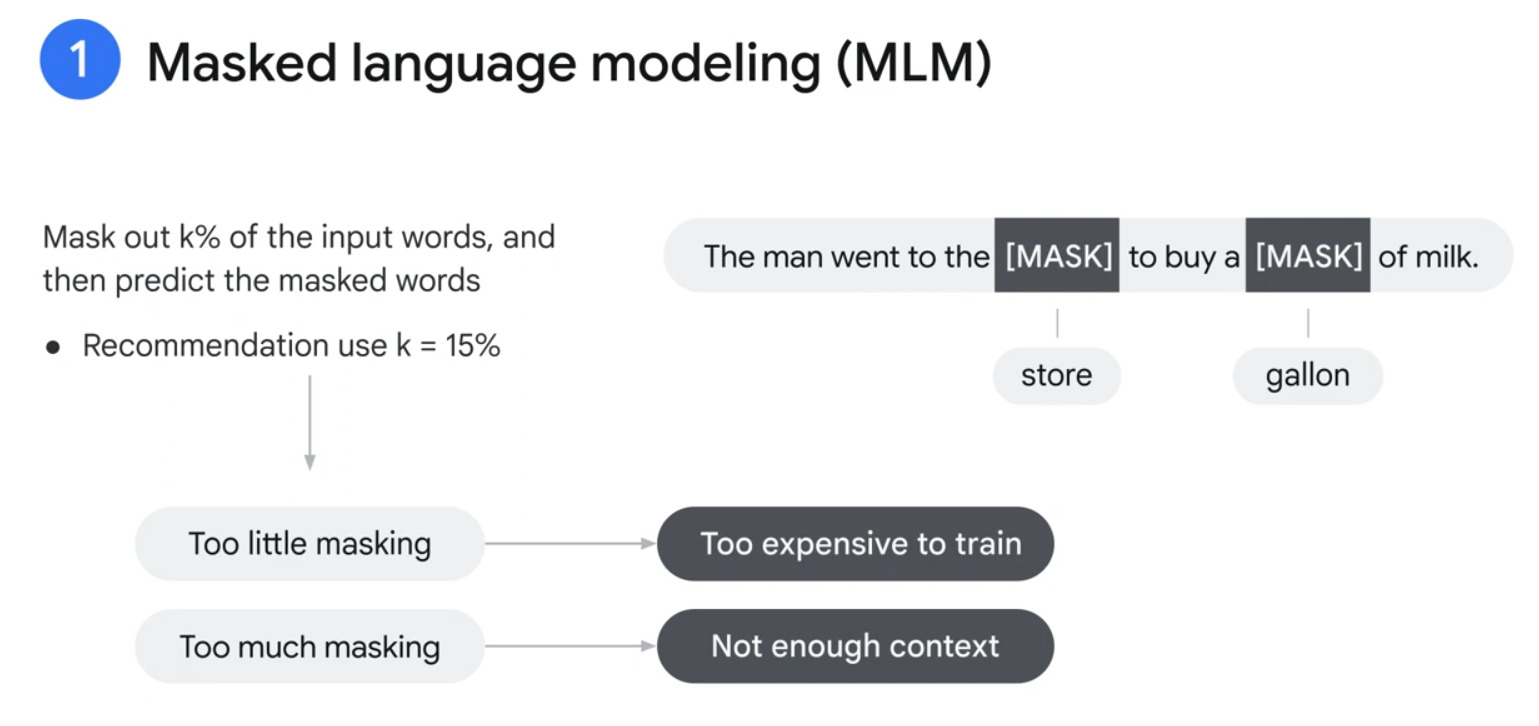
\includegraphics[width=0.9\textwidth]{bert1.jpeg}
                    \end{figure}
                \end{column}
                \begin{column}{0.5\textwidth}
                    \begin{figure}
                        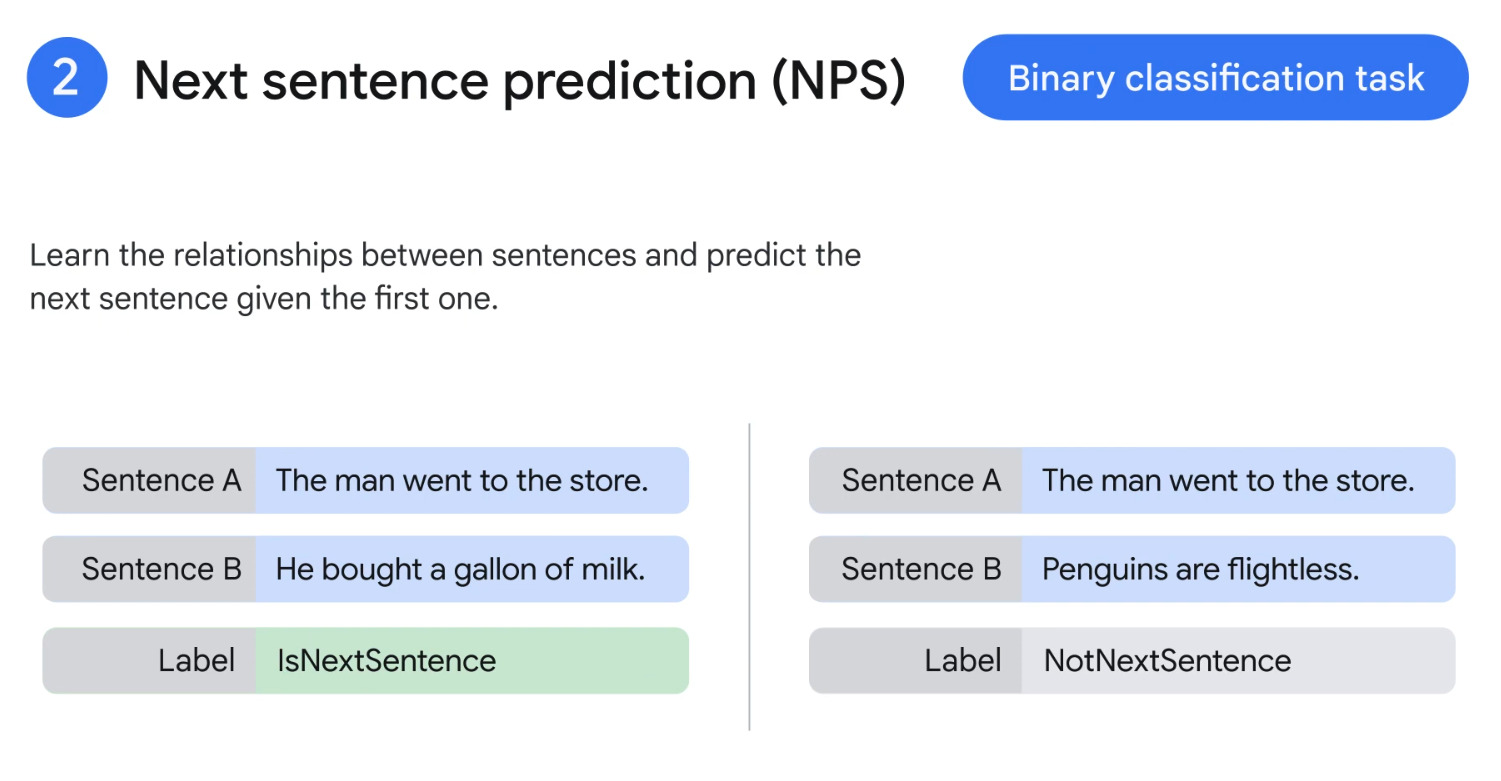
\includegraphics[width=0.9\textwidth]{bert2.jpeg}
                    \end{figure}
                \end{column}
            \end{columns}
            \footnotesize

            BERT uses a bi-directional approach considering both the left and
            right context of words in a sentence, instead of analyzing the text
            sequentially, BERT looks at all the words in a sentence
            simultaneously.

    \end{itemize}
\end{frame}

\begin{frame}{Background}
    \begin{itemize}
        \item BEiT (Bidirectional Encoder for Image Transformers):

            \begin{itemize}
            \item BEiT is a self-supervised vision representation model that uses a
            masked image modeling task to pretrain vision Transformers,
            achieving competitive results on downstream tasks like image
            classification and semantic segmentation.

            \item Unlike BERT, the BEiT model accepts continuous inputs so before pre-training,
            we learn an “image tokenizer” via autoencoding-style reconstruction, where an image is tokenized into
            discrete visual tokens according to the learned vocabulary.

        \item Labels of different image patches were defined using a Vector
            Quantized Variational AutoEncoder (VQ-VAE).
            A VQ-VAE uses an encoder to map a set of inputs to
            latent vectors, which are subsequently projected onto the
            nearest element within a finite codeboo
            \end{itemize}

    \end{itemize}
\end{frame}

\begin{frame}
    \begin{figure}
        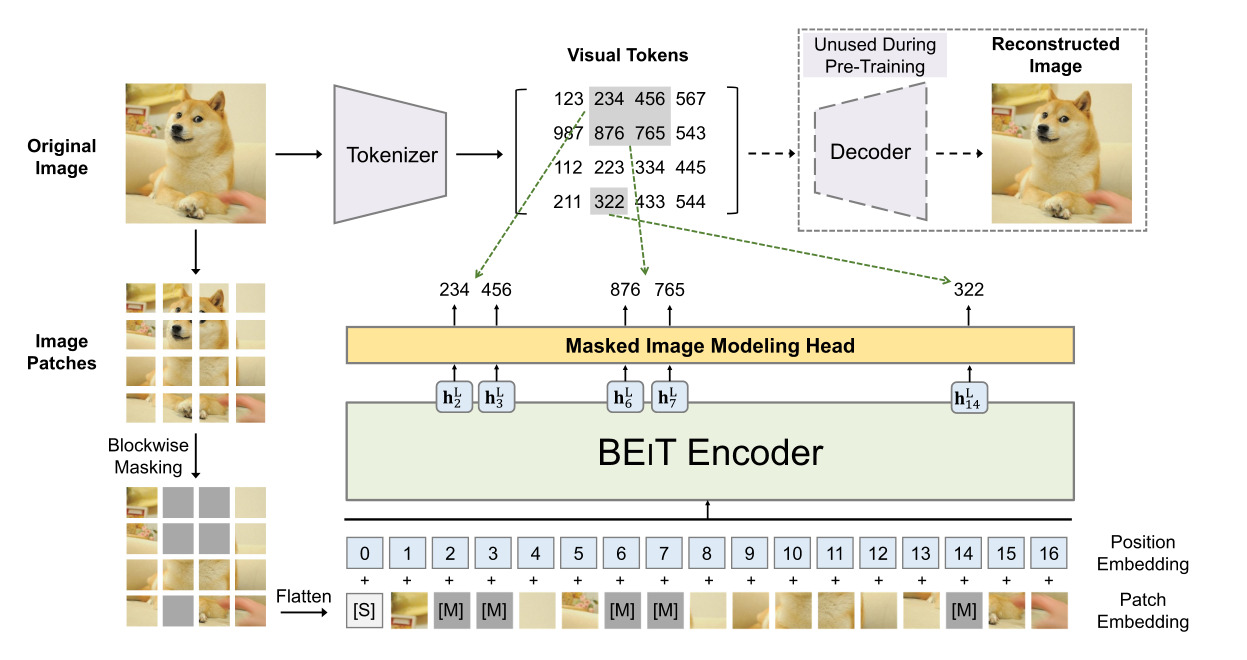
\includegraphics[width=0.9\textwidth]{beit.jpeg}
        \caption{Overview of BEiT pre-training. The patches are fed to a backbone vision
        Transformer. The pre-training task aims at predicting the visual tokens
    of the original image based
on the encoding vectors of the corrupted image}
\end{figure}
\end{frame}

\begin{frame}{Why we chose this approach?}

    \begin{itemize}[<+->]
        \item \textbf{Why not supervised models?}
Unlike supervised learning, which typically acquires limited domain representations
and focuses on a few key features for high prediction accuracy that must be learned anew for each task, SSL aims
to learn generic representations summarizing domain features that prove useful across various downstream tasks.
SSL tasks can be formulated on unlabeled data.
        \item \textbf{Why to mask the tokens?}
            In BERT the MLM model gave it a dramatic improvement over previous state-of-the-art
            models and served as on of the earliest examples of large language
            model.

           Traditional language models process text sequentially, either from
           left to right or right to left. This method limits the model’s
           awareness to the immediate context preceding the target word.

           By masking random tokens, the model is forced to use both left and
           right context to predict the masked word. This enables the model to
           learn bidirectional representations, unlike traditional left-to-right
           language model

   \end{itemize}
\end{frame}


\begin{frame}{Challenges in using HEP data for Foundation Models}

    The results from models in NLP seem promising, but there are a few
    fundamental problems in dataset in the context of HEP which differ
    the training scheme used, which need to be addressed:

    \begin{itemize}[<+->]
        \item \textbf{Tokenization}:
            Unlike language models, which operate on a finite and
            discrete vocabulary of words, many of the features one
            that describe particles are continuous, such as momentum,
            direction, distance of closest approach to the primary collision, etc.
            This changes the way we pass the input or parse the output when
            pre-training.
        \item \textbf{Permuation of datasets}:
            The particles in a jet don't have a specific order, so it makes
            sense to use a model that treats them all equally. However, if we
            replace all masked particles with the same placeholder, the model
            can't tell them apart. This means it would produce the same output
            for all masked particles, which isn't very useful. To avoid this
            problem, we need to either give the particles an order or add some
            way for them to interact with each other uniquely.
    \end{itemize}

\end{frame}

\begin{frame}{Tokenization Strategies}
    To tokenize the inputs the following methods have been experimented:
    \begin{enumerate}[<+->]
        \item Simple binning:
            Each feature is divided into a finite set of ranges, creating
            discrete bins.

            Limitation: Lacks contextual information about relationships between
            particles


        \item Vector Quantized Variational AutoEncoder (VQ-VAE):
            Uses an encoder to map inputs to latent vectors.
            Projects these vectors onto the nearest element in a finite
            codebook.
            Incorporates context from all input elements.
            Each particle is encoded to a single codebook element, considering
            all other particles in the jet.

            Limitation: More complex to implement and potentially
            computationally expensive


        \item K-means clustering:k
            Uses the K-means++ algorithm to define clusters.
            Each cluster is assigned an index, which is used as the target
            label.
            This method is context-independent, unlike the VQ-VAE approach

            Limitation: Context-independent, may miss important relationships
            between particles in a jet
    \end{enumerate}
\end{frame}

\begin{frame}{Ordering Strategies}
    The following ordering strategies have been experimented with:
    \begin{itemize}[<+->]
        \item \textbf{Ordering the input to the backbone:}
            Order particles by decreasing transverse momentum (pT) at
            the input stage of the model.

            \textbf{Limitation:} Breaks permutation invariance for all downstream tasks,
            which may adversely affect predictive performance.
        \item \textbf{Ordering only at the input to the pre-training prediction:}
            This method helps break symmetry for masked predictions without affecting the
            backbone's permutation invariance.

            Apply pT ordering just before the prediction head, using
            learned positional embeddings.

            \textbf{Limitation:} Adds complexity to the model architecture and may
            increase computational cost, though less severe than method 2.

    \end{itemize}
\end{frame}

\begin{frame}
    \begin{table}
        \centering
        \begin{tabular}{|l|l|l|l|}
            \hline
        \textbf{Ordering} & \textbf{Inputs} & \textbf{Loss}& \textbf{Accuracy} \\
            \hline
            no ordering & continuous & VQ-VAE classification & 54.1\% \\
            \textbf{order head} & \textbf{continuous} & \textbf{VQ-VAE
            classification} & \textbf{56.8\%} \\
            order backbone & continuous & VQ-VAE classification & 53.4\% \\
            order head & quantized & VQ-VAE classification & 51.1\% \\
            order head & quantized & K-means classification & 49.3\% \\
            order head & continuous & K-means classification & 56.2\% \\
            order head & continuous & regression & 48.9\% \\
            order backbone & continuous & regression & 46.3\% \\
            \hline
        \end{tabular}
        \caption{Comparison of different ordering strategies, input types, and
        loss functions}
        \label{table:comparison}
    \end{table}
\end{frame}


\begin{frame}{Masked Particle Modeling Objective}
    Let's say a jet is given by:
    $$ X = \{x_i\}_{i=1}^{N} \text{\hspace{1cm}($x_i$ represents a particle)} $$
    MPM partitions the set of particles in each jet in the dataset into masked and unmasked
    set:
    $$ \ma_x = \{x_i\}_{i\in \ma}, \hspace{0.5cm} \ua_x = \{x_i\}_{i\in \ua}$$

    The goal of pretraining is to find out a parametric function $f_\theta: X \to
    \mathbb{R}^{Nxd}$ (assume d-dimentional paramter set for each particle) such that the expectation of loss $\la$ can be minimized.

    $$ \mathbb{E}_x \left[ \frac{1}{|\ma_m|} \sum_{i\in \ma_m} \la(x_i,
    f_{\theta,i}(\ma_m, \ua_x)) \right] $$

\end{frame}

\begin{frame}{Overview diagram of MPM}
    \begin{figure}
        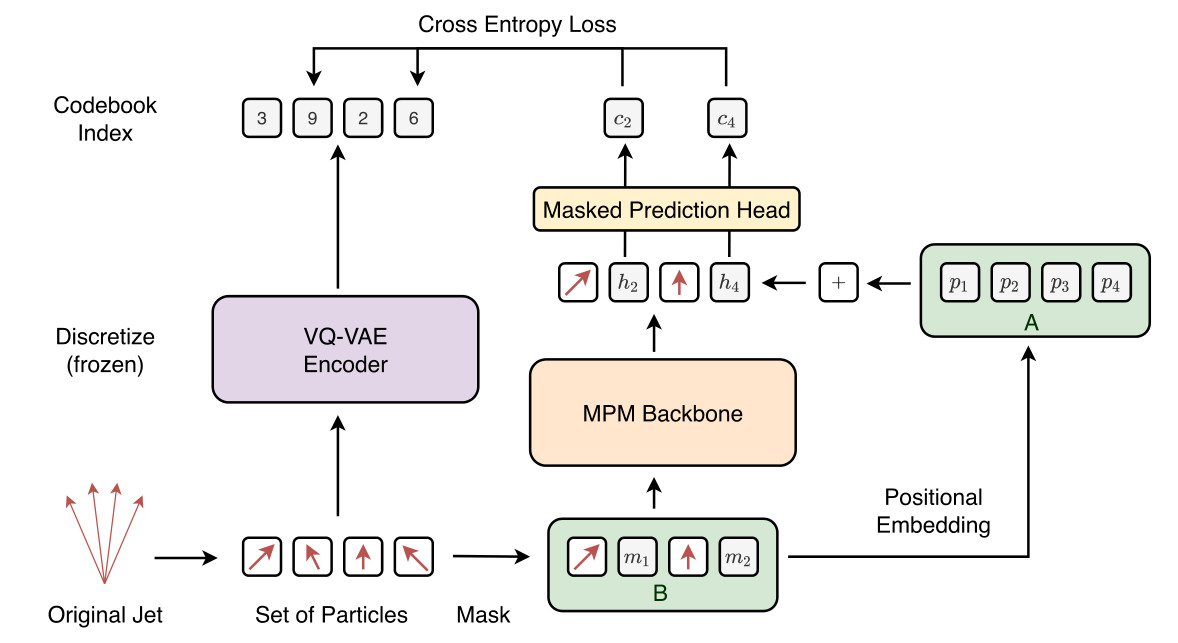
\includegraphics[width=0.8\textwidth]{mpm.jpeg}
    \end{figure}
\end{frame}

\begin{frame}{Datasets Used}

    \begin{enumerate}[<+->]
        \item
            \textbf{\href{https://zenodo.org/records/6619768}{JetClass Dataset:}} Used for pretraining the backbone
            \begin{itemize}
            \item It contains 100 million samples and has 10 different classes, with
            equal samples in each class. Examples include jets from Higgs boson
            decay, quarks, gluons, and other particles.
        \item Each class represents jets from different particle decays
        \item Uses particle momentum and direction as features
            \end{itemize}


        \item
        \textbf{\href{https://arxiv.org/abs/2408.11616}{RODEM Dataset:}} We are used as a test-set and for
            fine-tuning.
            \begin{itemize}
        \item Has 10 million samples for each class. Contains additional samples of top quark jets and combined
            quark/gluon jets.
        \item Uses slightly different parameters for jet clustering
            Covers a wider range of jet energies and directions
        \item Only uses particle's four momentum as feature, assuming particles are
            massless
            \end{itemize}
    \end{enumerate}

\end{frame}

\begin{frame}{Results}
    \textbf{Terminology:}
    \begin{itemize}[<+->]
        \item Fixed Backbone - The model just after the pretraining, without
            fine-tuning
        \item Fine-tuned Model - The pretrained backbone, is fine tuned for
            that specific downstream task.
        \item From-Scratch - Best Supervised model for that specific task
    \end{itemize}

    \begin{figure}
        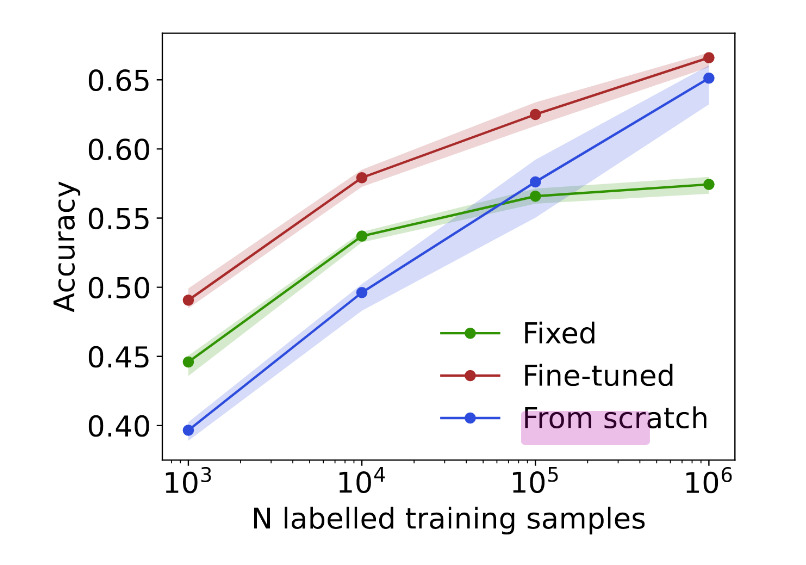
\includegraphics[width=0.4\textwidth]{plot1.jpeg}
        \caption{Accuracy of different training strategies as a
        function of the number of labelled training samples. Pretained in
    JetClass}
    \end{figure}
\end{frame}

\begin{frame}{Results}
    When tested and fine-tuned on a different dataset (RODEM), but pretained in
    JetClass:
    \begin{figure}
        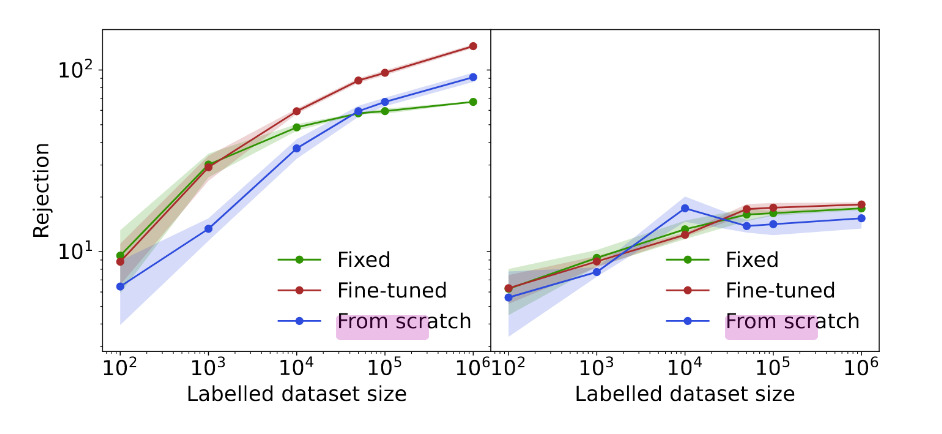
\includegraphics[width=0.8\textwidth]{plot2.jpeg}
        \caption{The QCD rejection
        evaluated on (left) the RODEM test set and (right) the
    JetClass test set, as a function of the size of the RODEM
data set used for fine-tuning}
    \end{figure}
\end{frame}


\begin{frame}{Conclusion}
         Masked particle modeling adapts well to unordered inputs in high
            energy physics.
    \begin{itemize}

         \item  Pre-trained models perform well on downstream tasks with minimal
                fine-tuning. Models generalize to unseen classes and show strong
                performance in weak supervision.
         \item  Pre-training on experimental data shows promise for
                addressing domain adaptation. Larger datasets for pretraining and better models may further improve
                performance in this field.


    \end{itemize}
\end{frame}


\AtBeginSection[]{
  \begin{frame}
  \vfill
  \centering
  \begin{beamercolorbox}[sep=8pt,center,shadow=false,rounded=true]{title}
    \usebeamerfont{title}\huge \insertsectionhead\par%
  \end{beamercolorbox}
  \vfill
  \end{frame}
}

\begin{frame}
  \begin{beamercolorbox}[sep=8pt,center,shadow=false,rounded=true]{title}
  \centering \Huge
  Thank You
  \end{beamercolorbox}
\end{frame}


\end{document}
